The robot model chosen for simulation was modeled after easily producible robots on the same scale.  The software driving the simulation was intended to be portable enough to work on a hardware implementation, and the model facilitates this goal as well.  Additionally, the robot model would have to be easily trainable and debuggable when implemented in hardware; use of a Geiger counter as an input would be unfavorable.  Lastly the sensors and design chosen had to facilitate the concept of natural learning, modeling after nature to some degree.

\subsection{Robot Inputs and Outputs}

Multiple inputs were modeled for simulation with outlets for control both by a human operator using sliders and by programmed handlers using a bridge class.  A microphone and light sensor were chosen as clear, human modifiable inputs that model after nature and could easily be used for reinforcement training.  An infrared light sensor was added as another easily controller variable in a testing setup: a human operator could easily bring closer and farther an IR LED for purposes of training.   Additionally sensors for battery level, three axes of accelerometers, and three axes of gyroscopes were added as more complex inputs for Fido to master.  The last sensor added was a three axis radio receiver.  The purpose of the receiver was to allow location based training of the robot relative to a radio beacon, such as following the beacon or avoiding it.  The radio sensor is a stand-in for Bluetooth, Wi-Fi, or any other radio technology; it is common practice in many areas of robotics to use radio beacons for localization.

\begin{figure}
	\centering
	\fbox{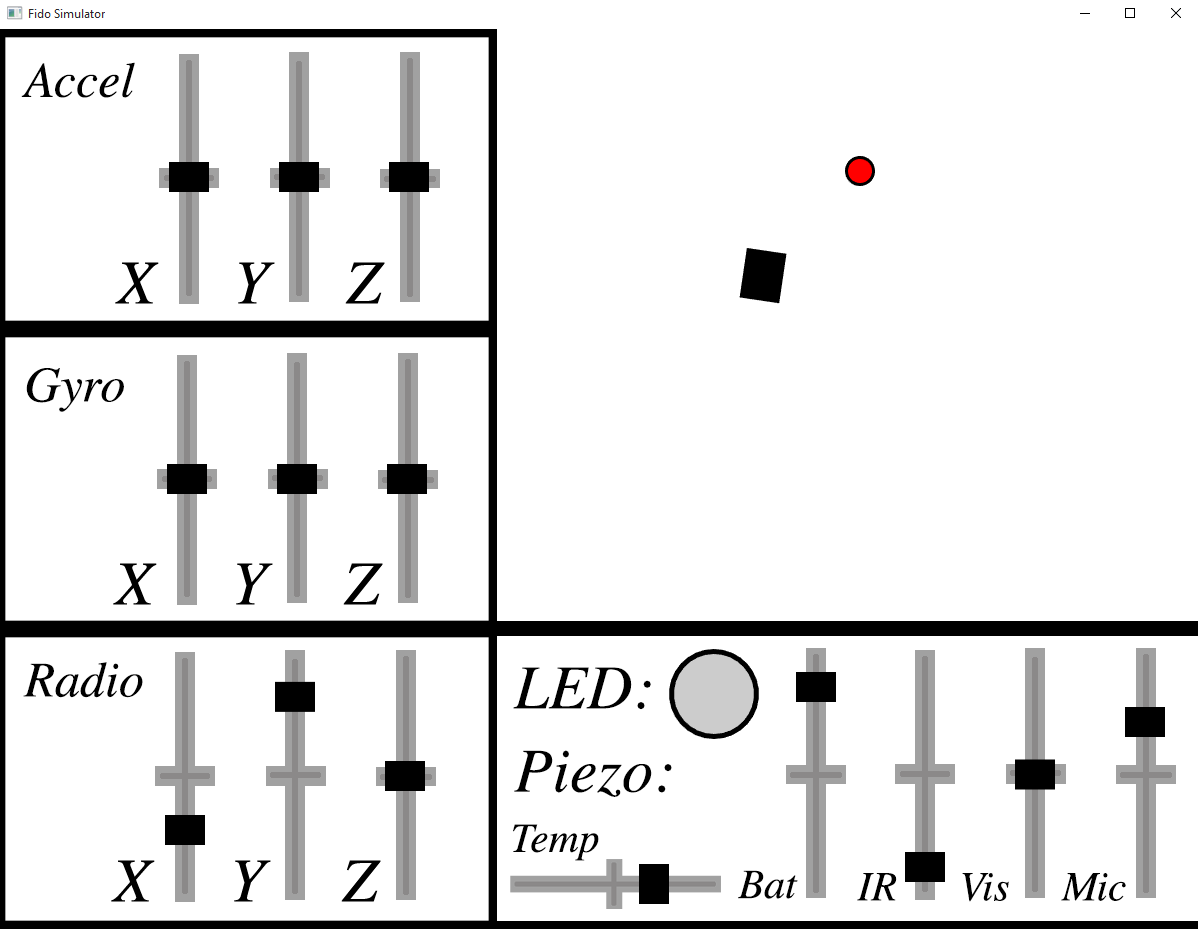
\includegraphics[height=10cm]{Figures/Screenshot.png}}
	\caption{Screenshot of Fido Simulator GUI}
\end{figure}

Fido's outputs were chosen similarly.  Two motors allow a drive mechanism known as differential drive, which will be discussed further in the following section.  A buzzer of varying tone and frequency and a multicolor LED complete the set of outputs.  

\subsection{Implementation and Kinematics}

A graphical user interface was made using the SFML multimedia library for C++.  Sliders manually adjust inputs such as accelerometer and gyroscope axes, battery life, and temperature.  A colored circle displays the output of the multicolor LED, while the frequency and volume of the piezoelectric speaker are displayed on the bottom bar.   Initially vectors of motor values were displayed graphically in the top right of the window.  This made sense for initial testing purposes: both competition entrants are experienced with differential drive robots, and can easily visualize robot movement from robot vectors.  However, as we decided to do more development on the simulator we wanted to allow more complex training on the simulator, such as path following.  Such training requires a visual kinematic simulation of the robot model.

\begin{figure}[ht]
	\centering
	\begin{tikzpicture}
	\begin{scope}[rotate=-20]
		\tikzset{dot/.style={circle,fill=#1,inner sep=0,minimum size=.5pt}}

		\draw[ultra thin] (0,0) -- (8,0);
		\draw[pattern=north west lines,thick](3,0) ellipse (0.4cm and 1.4cm);
		\draw[pattern=north west lines,thick](7,0) ellipse (0.4cm and 1.4cm);

		\node[circle,fill,inner sep=-2pt,label=below:${(x,y)}$] at (5,0){};
		\node[circle,fill,inner sep=-2pt,label={[xshift=.6cm, yshift=0.1cm]$\theta$}] at (0,0){};
		\node[circle,fill,inner sep=-2pt,label={[xshift=.2cm, yshift=-1.5cm]$\omega$}] at (0,0){};
		\node at (0,-.4) {ICC};

		\draw[->] (.5,0) arc (0:110:.5cm);
		\draw[->] (1,0) arc (0:-110:1cm);
		
		\draw[->] (2.3,-1) -- (2.3,1.5);
		\node at (1.8,.8) {$V_{left}$};
		\draw[->] (7.7,-1) -- (7.7,1.5);
		\node at (8.3,.8) {$V_{right}$};

		\draw[<->] (0,-2) -- (5,-2);
		\node at (2.5,-2.3) {$R$};

		\draw[<->] (3,2) -- (7,2);
		\node at (5,2.3) {$l$};
	\end{scope}
	
	\draw[step=.5cm,gray,ultra thin] (-1,1.5) grid (9,-4.5);
\end{tikzpicture}
	\caption{Differential Drive Kinematics Diagram}
\end{figure}

Fido's two motors are arranged in a differential drive arrangement.  Driving the left motor acts as a force vector on the left side of the robot, creating a torque around the right wheel.  The same applies with the right wheel.  When both motors are activated together, the motor drives straight.  Each motor has a value ranging from -100 to 100, where -100 is full power backwards, 0 is stopped, and 100 is full power forwards.   In order to transform motor values into a plottable transformation, we must first model the movement that our robot will take.

Every movement the robot takes can be interpreted as a rotation of radius $R$ around the ICC, or Instantaneous Center of Curvature.  If the robot is moving straight, this radius is simply infinite.   The robot travels at an angular velocity $\omega$ around the circle, and at any given moment is at the coordinates $(x,y)$ and orientation $\theta$.  The length of the robot from wheel-center to wheel-center is defined as $l$, while the velocity vectors of each motor are defined as $V_l$ and $V_r$ respectively.  The passing of time from the last call of motor values is defined as $\Delta t$.  We can solve for $R$ at any point using the following equation:

\begin{equation}
	R = \cfrac{l}{2} \times \cfrac{V_l + V_r}{V_r - V_l}\,.
\end{equation}

We can solve for $\omega$ using the following equation:

\begin{equation}
	\omega = \cfrac{V_r - V_l}{l}\,
\end{equation}

And the ICC location using the following equation:

\begin{equation}
	ICC = 
	\begin{bmatrix}
	    x - R\sin\theta\,, & y + R\cos\theta \\
	\end{bmatrix}
\end{equation}

We can then use these values to solve for the robot's new position, defined as coordinates $(x',y')$ and orientation $\theta'$.

\begin{equation}
	\begin{bmatrix}
	    x'      \\
	    y'      \\
	    \theta' \\
	\end{bmatrix} =
	\begin{bmatrix}
		\cos(\omega\Delta t) & -\sin(\omega\Delta t) & 0 \\
		\sin(\omega\Delta t) & \cos(\omega\Delta t)  & 0 \\
		0                    &                       & 1 \\
	\end{bmatrix}
	\begin{bmatrix}
		x - ICC_x  \\
		y - ICC_y  \\
		\theta     \\
	\end{bmatrix} + 
	\begin{bmatrix}
		ICC_x          \\
		ICC_y          \\
		\omega\Delta t \\
	\end{bmatrix}
\end{equation}

A brief inspection of these equations verify their performance in certain use cases.  If $V_r = -V_l$ $R$ becomes zero, as the robot turns around it's center.  If $V_r = V_l$ $R$ becomes infinite, as the robot is traveling in a straight line.   However the methodology by which the equation simplifies in the case of $V_r = V_l$ involves division of zero, which can be problematic in computer programming.   Therefore we must first check if $V_r = V_l$, and if so substitute an alternate equation as a simplification:

\begin{equation}
	\begin{bmatrix}
	    x'      \\
	    y'      \\
	    \theta' \\
	\end{bmatrix} =
	\begin{bmatrix}
	    x + V_l\Delta t \cos\Theta \\
	    y + V_l\Delta t \sin\Theta \\
	    \theta \\
	\end{bmatrix}
\end{equation}

The use of $V_l$ in this equation rather than $V_r$ is unimportant, as the values are equal.  Using these equations were were able to fully simulate Fido's kinematic model, and attach simulator motor inputs to Fido's outputs to visualize learning taking place.   The black rectangle in the upper right corner of the simulator is the robot, having been moved as part of training.  The red dot near the rectangle is a graphical representation of a radio beacon.  As adjusting sliders to represent the location of a radio beacon relative to the robot would be impractical, we decided to implement a beacon that could be placed and dragged by right clicking on the simulator.  Simulated sensor readings of beacon strength on two axis are gathered using an inverse square law, as applies to radio waves in general.  These readings are then displayed in the sliders and can be manually altered as well.  The radio beacon can be removed by a human operator by pressing the P key.  This has been especially helpful in the task of training Fido to follow a radio beacon.
